\documentclass[journal,12pt,twocolumn]{IEEEtran}
%
\usepackage{setspace}
\usepackage{gensymb}
\usepackage{xcolor}
\usepackage{caption}
%\usepackage{subcaption}
%\doublespacing
\singlespacing

%\usepackage{graphicx}
%\usepackage{amssymb}
%\usepackage{relsize}
\usepackage[cmex10]{amsmath}
\usepackage{mathtools}
%\usepackage{amsthm}
%\interdisplaylinepenalty=2500
%\savesymbol{iint}
%\usepackage{txfonts}
%\restoresymbol{TXF}{iint}
%\usepackage{wasysym}
\usepackage{hyperref}
\usepackage{amsthm}
\usepackage{mathrsfs}
\usepackage{txfonts}
\usepackage{stfloats}
\usepackage{cite}
\usepackage{cases}
\usepackage{subfig}
%\usepackage{xtab}
\usepackage{longtable}
\usepackage{multirow}
%\usepackage{algorithm}
%\usepackage{algpseudocode}
%\usepackage{enumerate}
\usepackage{enumitem}
\usepackage{mathtools}
%\usepackage{iithtlc}
%\usepackage[framemethod=tikz]{mdframed}
\usepackage{listings}
\let\vec\mathbf


%\usepackage{stmaryrd}


%\usepackage{wasysym}
%\newcounter{MYtempeqncnt}
\DeclareMathOperator*{\Res}{Res}
%\renewcommand{\baselinestretch}{2}
\renewcommand\thesection{\arabic{section}}
\renewcommand\thesubsection{\thesection.\arabic{subsection}}
\renewcommand\thesubsubsection{\thesubsection.\arabic{subsubsection}}

\renewcommand\thesectiondis{\arabic{section}}
\renewcommand\thesubsectiondis{\thesectiondis.\arabic{subsection}}
\renewcommand\thesubsubsectiondis{\thesubsectiondis.\arabic{subsubsection}}

%\renewcommand{\labelenumi}{\textbf{\theenumi}}
%\renewcommand{\theenumi}{P.\arabic{enumi}}

% correct bad hyphenation here
\hyphenation{op-tical net-works semi-conduc-tor}

\lstset{
	language=Python,
	frame=single, 
	breaklines=true,
	columns=fullflexible
}



\begin{document}
	%
	
	\theoremstyle{definition}
	\newtheorem{theorem}{Theorem}[section]
	\newtheorem{problem}{Problem}
	\newtheorem{proposition}{Proposition}[section]
	\newtheorem{lemma}{Lemma}[section]
	\newtheorem{corollary}[theorem]{Corollary}
	\newtheorem{example}{Example}[section]
	\newtheorem{definition}{Definition}[section]
	%\newtheorem{algorithm}{Algorithm}[section]
	%\newtheorem{cor}{Corollary}
	\newcommand{\BEQA}{\begin{eqnarray}}
		\newcommand{\EEQA}{\end{eqnarray}}
	\newcommand{\define}{\stackrel{\triangle}{=}}
	\newcommand{\myvec}[1]{\ensuremath{\begin{pmatrix}#1\end{pmatrix}}}
	\newcommand{\mydet}[1]{\ensuremath{\begin{vmatrix}#1\end{vmatrix}}}
	
	\bibliographystyle{IEEEtran}
	%\bibliographystyle{ieeetr}
	
	\providecommand{\nCr}[2]{\,^{#1}C_{#2}} % nCr
	\providecommand{\nPr}[2]{\,^{#1}P_{#2}} % nPr
	\providecommand{\mbf}{\mathbf}
	\providecommand{\pr}[1]{\ensuremath{\Pr\left(#1\right)}}
	\providecommand{\qfunc}[1]{\ensuremath{Q\left(#1\right)}}
	\providecommand{\sbrak}[1]{\ensuremath{{}\left[#1\right]}}
	\providecommand{\lsbrak}[1]{\ensuremath{{}\left[#1\right.}}
	\providecommand{\rsbrak}[1]{\ensuremath{{}\left.#1\right]}}
	\providecommand{\brak}[1]{\ensuremath{\left(#1\right)}}
	\providecommand{\lbrak}[1]{\ensuremath{\left(#1\right.}}
	\providecommand{\rbrak}[1]{\ensuremath{\left.#1\right)}}
	\providecommand{\cbrak}[1]{\ensuremath{\left\{#1\right\}}}
	\providecommand{\lcbrak}[1]{\ensuremath{\left\{#1\right.}}
	\providecommand{\rcbrak}[1]{\ensuremath{\left.#1\right\}}}
	\theoremstyle{remark}
	\newtheorem{rem}{Remark}
	\newcommand{\sgn}{\mathop{\mathrm{sgn}}}
	\providecommand{\abs}[1]{\left\vert#1\right\vert}
	\providecommand{\res}[1]{\Res\displaylimits_{#1}} 
	\providecommand{\norm}[1]{\lVert#1\rVert}
	\providecommand{\mtx}[1]{\mathbf{#1}}
	\providecommand{\mean}[1]{E\left[ #1 \right]}
	\providecommand{\fourier}{\overset{\mathcal{F}}{ \rightleftharpoons}}
	\providecommand{\ztrans}{\overset{\mathcal{Z}}{ \rightleftharpoons}}
	
	%\providecommand{\hilbert}{\overset{\mathcal{H}}{ \rightleftharpoons}}
	\providecommand{\system}{\overset{\mathcal{H}}{ \longleftrightarrow}}
	%\newcommand{\solution}[2]{\textbf{Solution:}{#1}}
	\newcommand{\solution}{\noindent \textbf{Solution: }}
	\providecommand{\dec}[2]{\ensuremath{\overset{#1}{\underset{#2}{\gtrless}}}}
	\numberwithin{equation}{section}
	%\numberwithin{equation}{subsection}
	%\numberwithin{problem}{subsection}
	%\numberwithin{definition}{subsection}
	
	%\renewcommand{\thefigure}{\theproblem.\arabic{figure}}
	\renewcommand{\thefigure}{\arabic{section}.\arabic{figure}}
	\makeatletter
	\@addtoreset{figure}{section}
	\makeatother
	
	%\numberwithin{figure}{subsection}
	
	\def\putbox#1#2#3{\makebox[0in][l]{\makebox[#1][l]{}\raisebox{\baselineskip}[0in][0in]{\raisebox{#2}[0in][0in]{#3}}}}
	\def\rightbox#1{\makebox[0in][r]{#1}}
	\def\centbox#1{\makebox[0in]{#1}}
	\def\topbox#1{\raisebox{-\baselineskip}[0in][0in]{#1}}
	\def\midbox#1{\raisebox{-0.5\baselineskip}[0in][0in]{#1}}
	
	\vspace{3cm}
	
	\title{ 
		%\logo{
			%}
		Pingala Series
		%	\logo{Octave for Math Computing }
	}
	%\title{
		%	\logo{Matrix Analysis through Octave}{\begin{center}\includegraphics[scale=.24]{tlc}\end{center}}{}{HAMDSP}
		%}
	
	
	% paper title
	% can use linebreaks \\ within to get better formatting as desired
	%\title{Matrix Analysis through Octave}
	%
	%
	% author names and IEEE memberships
	% note positions of commas and nonbreaking spaces ( ~ ) LaTeX will not break
	% a structure at a ~ so this keeps an author's name from being broken across
	% two lines.
	% use \thanks{} to gain access to the first footnote area
	% a separate \thanks must be used for each paragraph as LaTeX2e's \thanks
	% was not built to handle multiple paragraphs
	%
	
	\author{Dhanush Pittala\\BM20BTECH11004}
	
	% make the title area
	\maketitle
	
	%\newpage
	
	\tableofcontents
	
	\bigskip
	
	\begin{abstract}
		This manual provides a simple introduction to Transforms
	\end{abstract}
	\section{JEE 2019}
	\noindent Let $\alpha$ and $\beta$ ($\alpha > \beta$) be the roots of the
	equation $z^2 - z - 1 = 0$. Define,
	\begin{align}
		a_n &= \frac{\alpha^{n}-\beta^{n}}{\alpha - \beta}, \quad n \ge 1
		\\
		b_n &= a_{n-1} + a_{n+1}, \quad n \ge 2, \quad b_1 =1
		\label{eq:10-orig-diff}
	\end{align}
	Verify the following using a python code.
	\begin{enumerate}[label=\thesection.\arabic*
		,ref=\thesection.\theenumi]
		\item 
		\begin{align}
			\sum_{k=1}^{n}a_k = a_{n+2}-1, \quad n \ge 1
		\end{align}
		\item 
		\begin{align}
			\sum_{k=1}^{\infty}\frac{a_k}{10^k} =\frac{10}{89}
		\end{align}
		\item 
		\begin{align}
			b_n =\alpha^n + \beta^n, \quad n \ge 1
		\end{align}
		\item 
		\begin{align}
			\sum_{k=1}^{\infty}\frac{b_k}{10^k} =\frac{8}{89}
		\end{align}
	\end{enumerate}
	Download the Python code using
	\begin{lstlisting}
		wget https://github.com/dhanushpittala11/EE3900-2022/blob/main/pingala/codes/pingala1.1.ipynb
	\end{lstlisting}
	\section{Pingala Series}
	\begin{enumerate}[label=\thesection.\arabic*,ref=\thesection.\theenumi]
		\item The {\em one sided} $Z$-transform of $x(n)$ is defined as 
		\begin{align}
			X^{+}(z) = \sum_{n = 0}^{\infty}x(n)z^{-n}, \quad z \in \mathbb{C}
			\label{eq:one-Z}
		\end{align}
		\item The {\em Pingala} series is generated using the difference equation 
		\begin{align}
			x(n+2) = x\brak{n+1} + x\brak{n},  \quad x(0) = x(1) = 1, n \ge 0
			\label{eq:10-pingala}
		\end{align}
		Generate a stem plot for $x(n)$.
		
		\solution
		Download the Python code
		\begin{lstlisting}
			wget https://github.com/dhanushpittala11/EE3900-2022/blob/main/pingala/codes/pingala2.1.ipynb
		\end{lstlisting}
		\begin{figure}[!htp]
			\includegraphics[width=\columnwidth]{/home/dhanush/Pictures/Screenshots/2.1.png}
			\caption{Plot of $x(n)$}
			\label{fig:xn}
		\end{figure}
		
		\newpage
		\item Find $X^{+}(z)$.
		
		\solution Taking the one-sided $Z$-transform on both sides of \eqref{eq:10-pingala},
		\begin{align}
			&\mathcal{Z}^+\sbrak{x(n + 2)} = \mathcal{Z}^+\sbrak{x(n + 1)} + \mathcal{Z}^+\sbrak{x(n)} \\
			&z^2X^+(z) - z^2x(0) - zx(1) = zX^+(z) - zx(0) + zX^+(z) \\
			&\brak{z^2 - z - 1}X^+(z) = z^2 \\
			&X^+(z) = \frac{1}{1 - z^{-1} - z^{-2}} \\
			&= \frac{1}{\brak{1 - \alpha z^{-1}}\brak{1 - \beta z^{-1}}}, \quad |z| > \alpha
			\label{eq:X-z}
		\end{align}
		\item Find $x(n)$.
		
		\solution Expanding $X^+(z)$ in \eqref{eq:X-z} using partial fractions, we get
		\begin{align}
			X^+(z) &= \frac{1}{\brak{\alpha - \beta}z^{-1}}\sbrak{\frac{1}{1 - \alpha z^{-1}} - \frac{1}{1 - \beta z^{-1}}} \\
			&= \frac{1}{\brak{\alpha - \beta}}\sum_{n = 0}^{\infty}\brak{\alpha^n - \beta^n}z^{-n + 1} \\
			&= \sum_{n = 1}^{\infty}\frac{\alpha^{n} - \beta^{n}}{\alpha - \beta}z^{-n + 1} \\
			&= \sum_{k = 0}^{\infty}\frac{\alpha^{k + 1} - \beta^{k + 1}}{\alpha - \beta}z^{-k}
		\end{align}
		where $k := n + 1$. Thus,
		\begin{align}
			x(n) = \frac{\alpha^{n + 1} - \beta^{n + 1}}{\alpha - \beta}u(n) = a_{n + 1}u(n)
			\label{eq:x-n-def}
		\end{align}
		\item Sketch 
		\begin{align}
			y(n) = x\brak{n-1} + x\brak{n+1},  \quad n \ge 0
			\label{eq:10-orig-diff-rev}
		\end{align}
		
		\solution
		Download the Python code using
		\begin{lstlisting}
			wget https://github.com/dhanushpittala11/EE3900-2022/blob/main/pingala/codes/pingala2.2.ipynb
		\end{lstlisting}
		\begin{figure}[!htbp]
			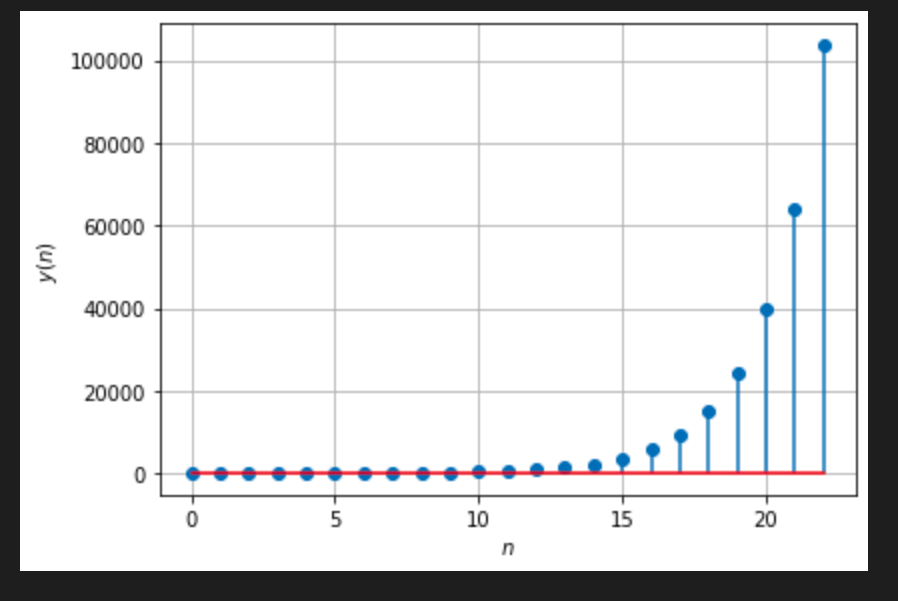
\includegraphics[width=\columnwidth]{/home/dhanush/Pictures/Screenshots/2.2.png}
			\caption{Plot of $y(n)$}
			\label{fig:yn}
		\end{figure}
		\item Find $Y^{+}(z)$. 
		
		\solution Taking the one-sided $Z$-transform on both sides of \eqref{eq:10-orig-diff-rev},
		\begin{align}
			&\mathcal{Z}^+\sbrak{y(n)} = \mathcal{Z}^+\sbrak{x(n + 1)} + \mathcal{Z}^+\sbrak{x(n - 1)} \\
			&Y^+(z) = zX^+(z) - zx(0) + z^{-1}X^+(z) + zx(-1) \\
			&= \frac{z + z^{-1}}{1 - z^{-1} - z^{-2}} - z \\
			&= \frac{1 + 2z^{-1}}{1 - z^{-1} - z^{-2}}, \quad |z| > \alpha
		\end{align}
		since $x(n) = 0\ \forall\ n < 0$.
		\item Find $y(n)$.
		\label{pr:1-3}
		
		\solution Using \eqref{eq:X-z},
		\begin{align}
			Y^+(z) &= (1 + 2z^{-1})\sum_{n = 0}^{\infty}x(n)z^{-n} \\
			&= \sum_{n = 0}^{\infty}x(n)z^{-n} + \sum_{n = 1}^{\infty}2x(n - 1)z^{-n} \\
			&= x(0) + \sum_{n = 1}^{\infty}\brak{x(n) + 2x(n - 1)}z^{-n}
		\end{align}
		Thus, $y(0) = x(0) = 1$ and for $n \ge 1$, using the fact that $\alpha$ and 
		$\beta$ are the roots of the equation $z^2 - z - 1 = 0$,
		\begin{align}
			y(n) &= \frac{\brak{\alpha^{n + 1} - \beta^{n + 1}} + \brak{2\alpha^n + 2\beta^n}}{\alpha - \beta} \\
			&= \frac{\brak{\alpha^{n + 2} - \beta^{n + 2}} + \brak{\alpha^{n} + \beta^{n}}}{\alpha - \beta} \label{eq:y-b} \\
			&= \frac{\brak{\alpha^{n + 2} - \beta^{n + 2}} - \alpha\beta\brak{\alpha^{n} + \beta^{n}}}{\alpha - \beta} \\
			&= \frac{\brak{\alpha - \beta}\brak{\alpha^{n + 1} + \beta^{n + 1}}}{\alpha - \beta} \\
			&= \alpha^{n + 1} + \beta^{n + 1}
		\end{align}
		Thus, $y(n) = \alpha^{n + 1} + \beta^{n + 1}$ for $n \geq 0$ as $\alpha + \beta = 1$.
		Comparing \eqref{eq:y-b} with the definition of $b_n$, we see that $y(n) = b_{n + 1}$.
		Hence, $b_n = \alpha^n + \beta^n$.
	\end{enumerate}
	\section{Power of the Z transform}
	\begin{enumerate}[label=\thesection.\arabic*,ref=\thesection.\theenumi]
		\item Show that 
		\begin{align}
			\sum_{k=1}^{n}a_k = 
			\sum_{k=0}^{n-1}x(k) = x(n)*u(n-1)
		\end{align}
		
		\solution From \eqref{eq:x-n-def}, and noting that $x(n) = 0\ \forall\ n < 0$,
		\begin{align}
			\sum_{k=1}^{n}a_k &= \sum_{k=0}^{n-1}x(k) \\
			&= \sum_{k = -\infty}^{n - 1}x(k) \\
			&= \sum_{k = -\infty}^{\infty}x(k)u(n - 1 - k) \\
			&= x(n)*u(n - 1)
		\end{align}
		\item Show that 
		\begin{align}
			a_{n+2}-1, \quad n \ge 1
		\end{align}
		can be expressed as 
		\begin{align}
			\sbrak{x\brak{n+1}-1}u\brak{n}
		\end{align}
		
		\solution From \eqref{eq:x-n-def},
		\begin{align}
			a_{n+2} - 1 = \sbrak{x(n + 1) - 1}, \quad n \ge 0
		\end{align}
		and so, using the definition of $u(n)$,
		\begin{align}
			a_{n+2} - 1 = \sbrak{x(n + 1) - 1}u(n)
		\end{align}
		
		\item Show that 
		\begin{align}
			\sum_{k=1}^{\infty}\frac{a_k}{10^k}= 
			\frac{1}{10}\sum_{k=0}^{\infty}\frac{x\brak{k}}{10^k} =\frac{1}{10}X^{+}\brak{{10}}
		\end{align}
		\label{pr:1-2}
		\solution 
		\begin{align}
			\sum_{k=1}^{\infty}\frac{a_k}{10^k} &= \frac{1}{10}\sum_{k = 0}^{\infty}\frac{a_{k+1}}{10^k} \\
			&= \frac{1}{10}\sum_{k = 0}^{\infty}\frac{x(k)}{10^k} \\
			&= \frac{1}{10}X^+(z) \\
			&= \frac{1}{10}\times\frac{100}{89} = \frac{10}{89}
		\end{align}
		\item Show that 
		\begin{align}
			\alpha^n + \beta^n, \quad n \ge 1
			\label{eq:yn-exp}
		\end{align}
		can be expressed as 
		\begin{align}
			w(n) = \brak{\alpha^{n+1} + \beta^{n+1}}u(n)
		\end{align}
		and find $W(z)$.
		
		\solution Putting $n = k + 1$ in \eqref{eq:yn-exp} and using the definition of $u(n)$, 
		\begin{align}
			\alpha^n + \beta^n = \brak{\alpha^{k + 1} + \beta^{k + 1}}u(k)
		\end{align}
		Hence, \eqref{eq:yn-exp} can be expressed as
		\begin{align}
			w(n) = \brak{\alpha^{n+1} + \beta^{n+1}}u(n) = y(n)
		\end{align}
		Therefore,
		\begin{align}
			W(z) = Y(z) = \frac{1 + 2z^{-1}}{1 - z^{-1} - z^{-2}}
		\end{align}
		\item Show that 
		\begin{align}
			\sum_{k=1}^{\infty}\frac{b_k}{10^k} =
			\frac{1}{10}\sum_{k=0}^{\infty}\frac{y\brak{k}}{10^k} =\frac{1}{10}Y^{+}\brak{{10}}
		\end{align}
		\label{pr:1-4}
		\solution
		\begin{align}
			\sum_{k=1}^{\infty}\frac{b_k}{10^k} &= \frac{1}{10}\sum_{k = 0}^{\infty}\frac{b_{k+1}}{10^k} \\
			&= \frac{1}{10}\sum_{k = 0}^{\infty}\frac{y(k)}{10^k} \\
			&= \frac{1}{10}Y^+(z) \\
			&= \frac{1}{10}\times\frac{120}{89} = \frac{12}{89}
		\end{align}
		\item Solve the JEE 2019 problem.
		
		\solution We know that
		\begin{align}
			\sum_{k = 1}^{n}a_k = x(n)*u(n - 1)
		\end{align}
		But
		\begin{align}
			&x(n)*u(n - 1) \ztrans X(z)z^{-1}U(z) \\
			&= \frac{z^{-1}}{\brak{1 - z^{-1} - z^{-2}}\brak{1 - z^{-1}}} \\
			&= z\sbrak{\frac{1}{1 - z^{-1} - z^{-2}} - \frac{1}{1 - z^{-1}}} \\
			&\ztrans z\sum_{n = 0}^{\infty}\brak{x(n) - 1}z^{-n} \\
			&= \sum_{n = 0}^{\infty}\brak{x(n) - 1}z^{-n + 1} \\
			&= \sum_{n = 0}^{\infty}\brak{x(n + 1) - 1}z^{-n} \\
		\end{align}
		From \eqref{eq:x-n-def}, we get
		\begin{align}
			\sum_{k = 1}^{n}a_k = a_{n+2} - 1
		\end{align}
		We have already established the remaining options in order in the problems
		\eqref{pr:1-2}, \eqref{pr:1-3}, \eqref{pr:1-4}. Therefore, options 1, 2,
		and 3 are correct and option 4 is incorrect.
	\end{enumerate}
\end{document}